\section{Implementation}\label{implementation}

This section presents an implementation with the aim of improving the underwater color depthmap image generated by Raytrix. Previous work trying to improve the color depthmap image is shortly presented and discussed. The new implementation is explained step-by-step followed by images showing the process and result.


\subsection{Previous Work on the Depthmap Image}

Before the start of this project, setup of all needed hardware and software was already accomplished. Also, some implementation had already been made along with some experimental enhancement on the depthmap image.

As explained earlier, the Raytrix needs to be attached to a computer with the Raytrix software installed. One difficulty working with the Raytrix is that all 3D information is stored in its own raytrix format, which is not compatible with other processing tools. This format cannot be directly converted to PNG or JPG for further processing, but an implementation performing this conversion was already accomplished for the color depthmap image. The resulting color depthmap image in PNG format does not have any direct depth information, but consists of colors that only represent depth together with the Raytrix calibration.
However, the color depthmap is intuitive to work with, as it is clear to see the object's shape based on colors.

There was also some existing implementation for improving the color depthmap. One of these implementations evolved around interpolation algorithms. This was way too slow and did not give sufficient results, as the colors along the fish were not evenly distributed.  
Another implementation used simple filtering methods to remove particles too close or too far away from the object. For filling in missing color data an averaging filter was used. Also, the largest contour in the image was found, and the rest removed. This method was better in speed, but the results were still not sufficient. Figure \ref{fig:sealab_implementation} shows the result from this implementation.


\begin{figure}[H]
    \centering
    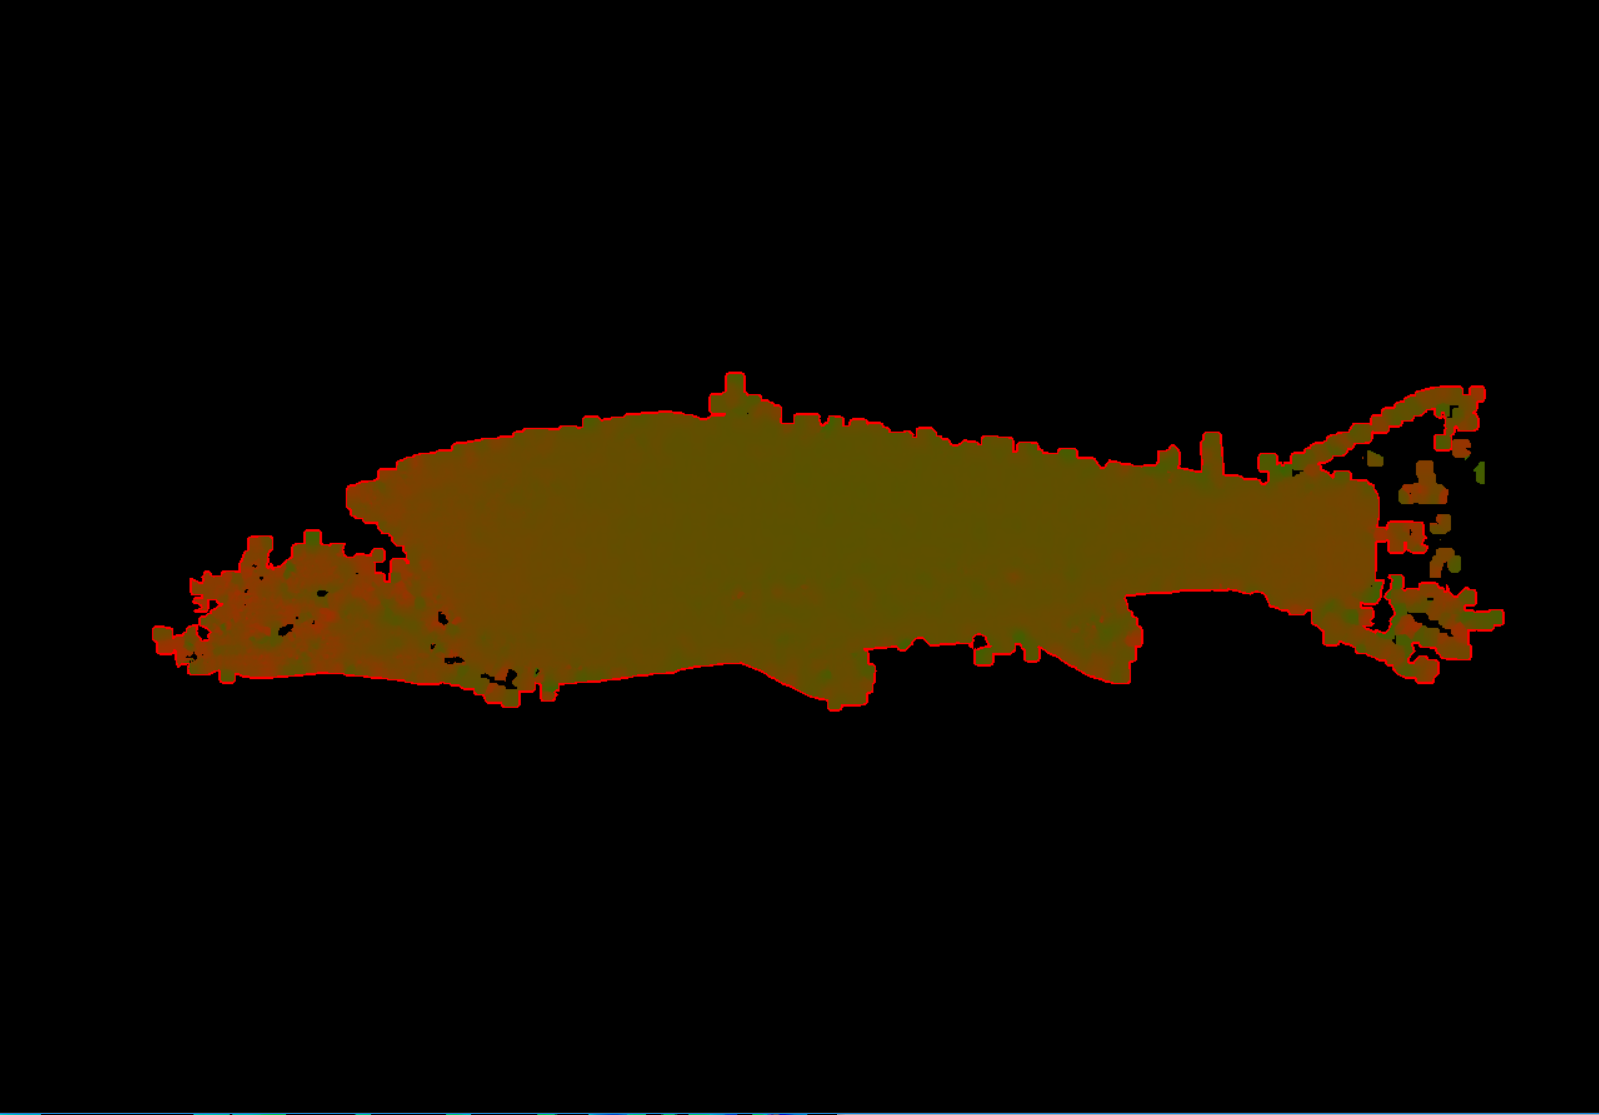
\includegraphics[width=.9\linewidth]{images/implementation/sealab_fish1}
    \caption{Previous Improvement of Color Depthmap}
    \label{fig:sealab_implementation}
\end{figure}


%%%%%%%%%%%%%%%%%%%%%%%%%%%%%%%%%%%%%%%%%%%%%%%%%%%%%%%%%%%%%%%%%%%%%%


\subsection{Depthmap Enhancement} \label{section:depthmap}

The approach used to better the depthmap image is mostly based on color filtering followed by morphological closing together with object detection. 
Color filtering is first used to remove detected particles. All data, based on its color, too close to the camera or too far behind the object is removed. This is an easy way of filtering out irrelevant data. Morphological closing is a very good operation for leveling out the color and fill the holes, and it is therefore used several times in a row on the color filtered image. The only problem is that the object will lose its original shape when run several iterations in a row. To solve this problem, an object detection algorithm was run on the color-filtered image. This algorithm finds the largest contour in the image and returns a binary mask of the contour. This mask is put on top of the morphologically closed image and makes the result.

It is assumed that the object in the depthmap has a smooth surface so that the depth data does not vary too much. It is also assumed only one object in each image, and that the object is centered in the detection area.

The steps of the algorithm follows below, and the complete code can be found in section \ref{code}.
\newpage

\begin{enumerate}
    \item \textbf{Filter out unwanted colors:}
    Color filtering was achieved by looping through each pixel in the image and setting it to black if its blue-value was too high, green-value too low or red-value too low. This removed all particles detected by the Raytrix that was too close or to far behind the object of interest, assuming the object is centered.
    
    \item \textbf{Remove small particles:}
    Removal of small particles was achieved by the use of morphological opening. Too much opening would remove much of the object, so here there is a fine line depending on how much color depth data is available on the object.
    
    \item \textbf{Find largest contour:} 
    Finding the largest contour followed these steps: 
    \begin{enumerate}[label*=\arabic*.]
        \item Convert to grayscale and normalize
        \item Sobel edge detector and thresholding
        \item Dilate
        \item Floodfill
        \item Erode
        \item Find largest contour
    \end{enumerate}
    This algorithm is found on GitHub \cite{website:largest_contour_code_github}, but has been modified. For further explanation of the complete algorithm, see \cite{website:largest_contour_code_explanation}.
    The resulting images for each step of the algorithm is shown in figure \ref{fig:find_largest_contour}.
    
    \item \textbf{Morphological closing on color-filtered image:}
    To fill out holes in the object in an even way, morphological closing was used. This also levels out the depth data on the surface of the object, such that small errors are removed.
    
    \item \textbf{Mask the morphological closed image with the largest contour:}
    Because the morphological closing operation somewhere expands the object, the largest contour was used as a mask to gain the final result. 
\end{enumerate}

Figure \ref{fig:algorithm} shows the given result after each step of the algorithm, where \ref{fig:masked_source} is the final result.


\begin{figure}[H]
    \begin{subfigure}{0.49\textwidth}
        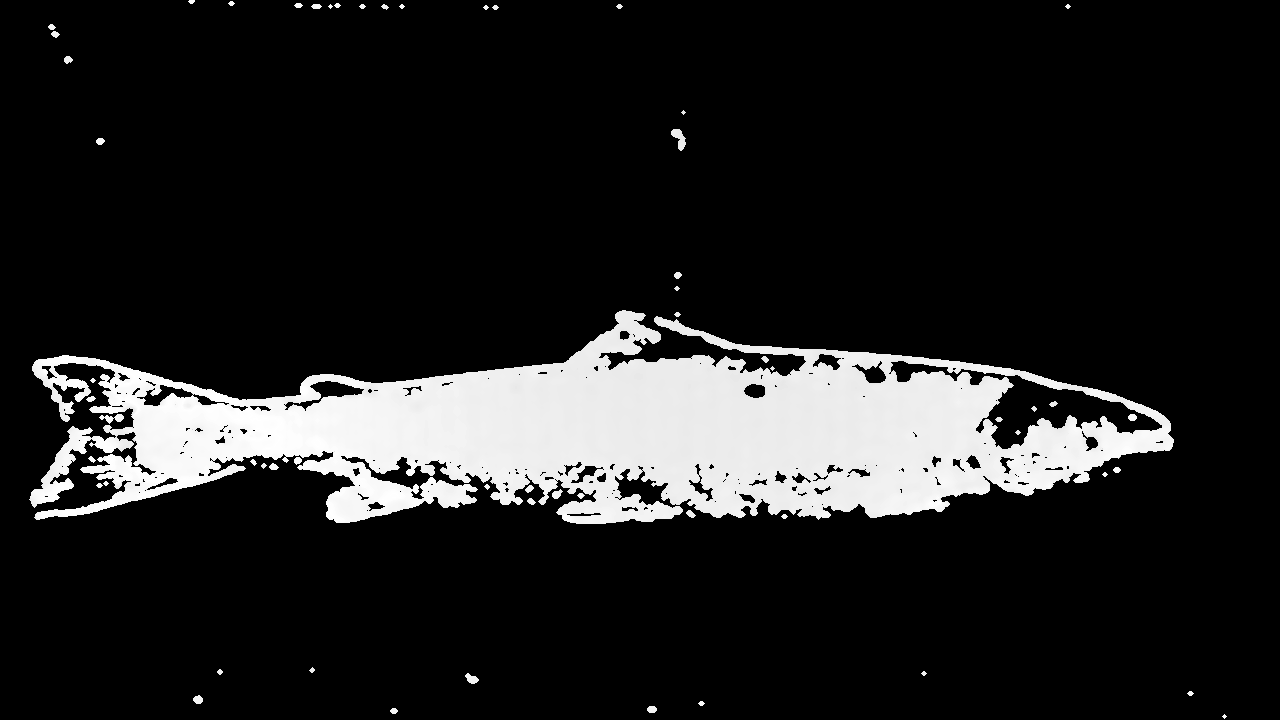
\includegraphics[width=\linewidth]{images/implementation/4_1_grayscale}
        \caption{Converted to Grayscale} 
        \label{fig:grayscale}
    \end{subfigure}\hspace*{\fill}
    \begin{subfigure}{0.49\textwidth}
        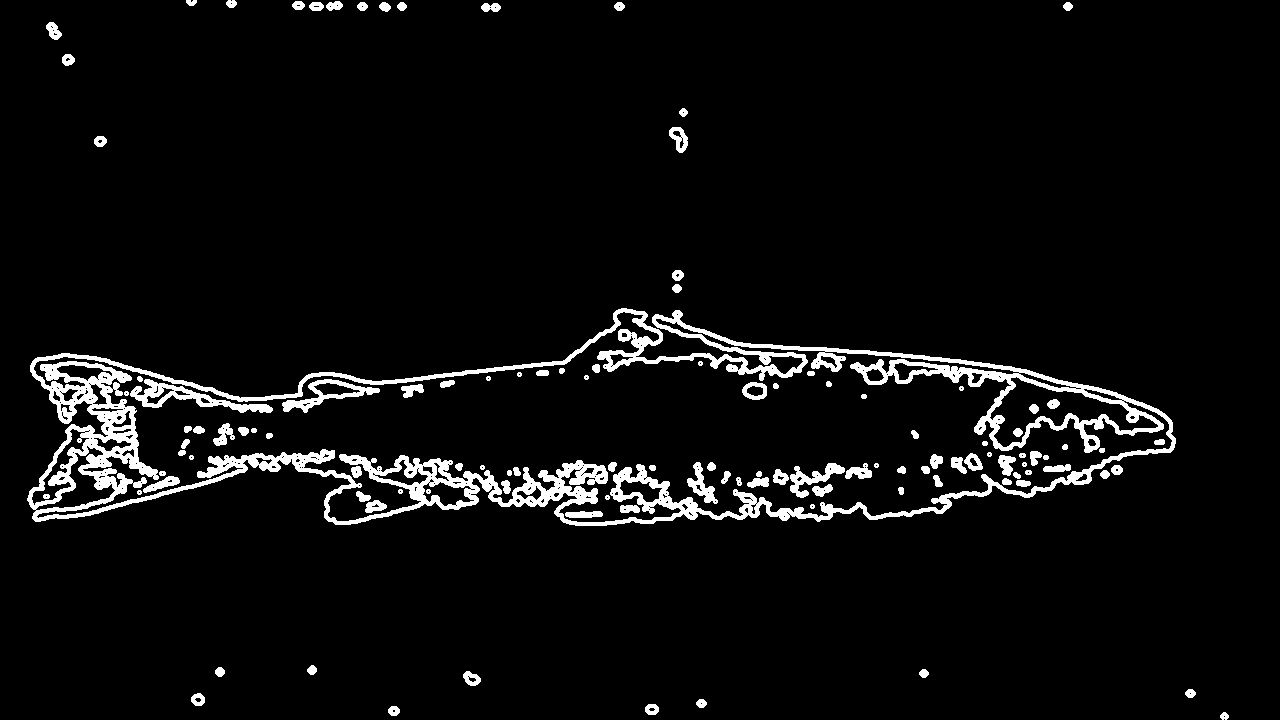
\includegraphics[width=\linewidth]{images/implementation/4_2_edge_detector}
        \caption{Edge Detection} 
        \label{fig:edge_detection}
    \end{subfigure}
    
    \medskip
    \begin{subfigure}{0.49\textwidth}
        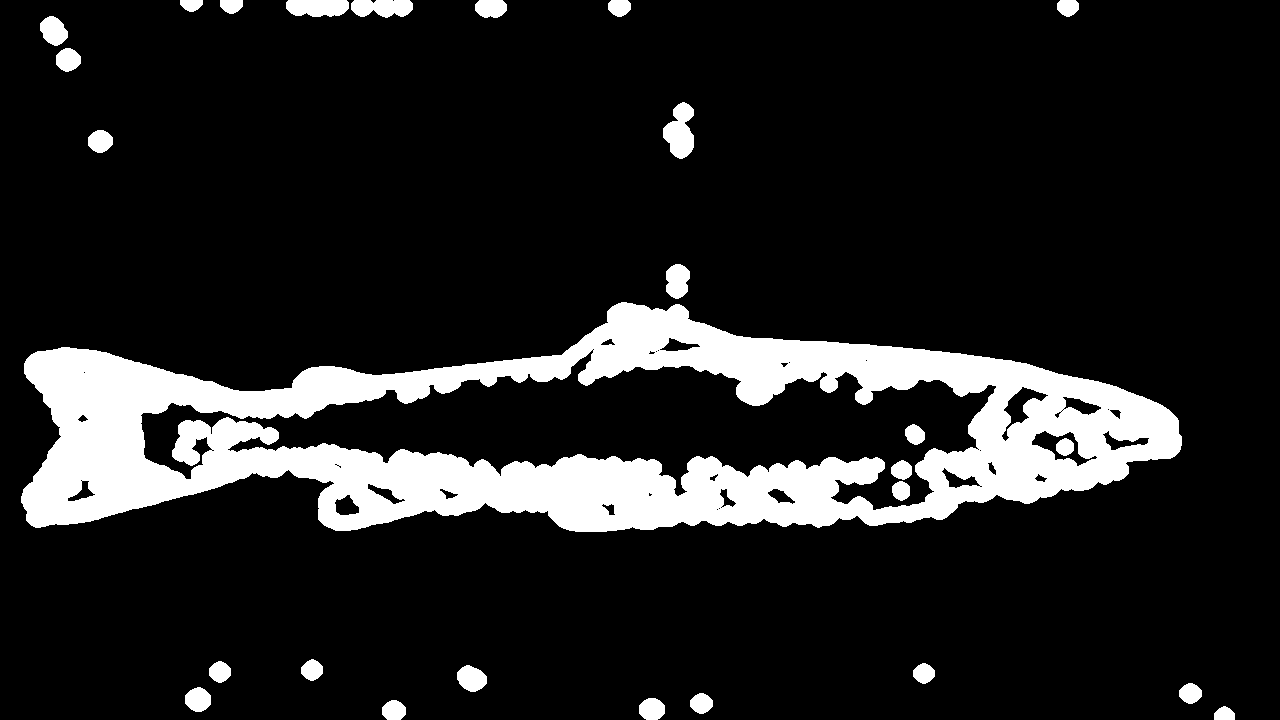
\includegraphics[width=\linewidth]{images/implementation/4_3_dilate}
        \caption{Dilate} 
        \label{fig:dilate_contour}
    \end{subfigure}\hspace*{\fill}
    \begin{subfigure}{0.49\textwidth}
        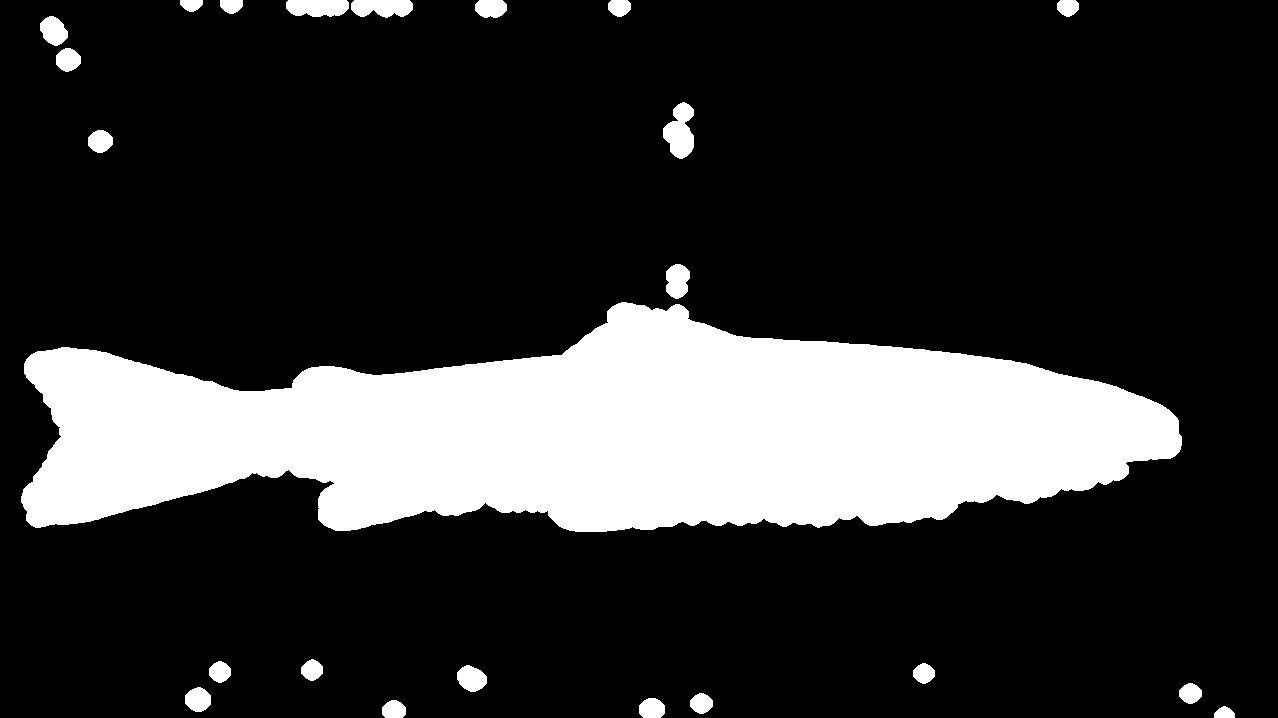
\includegraphics[width=\linewidth]{images/implementation/4_4_floodfill}
        \caption{Floodfill} 
        \label{fig:floodfill}
    \end{subfigure}
    
    \medskip
    \begin{subfigure}{0.49\textwidth}
        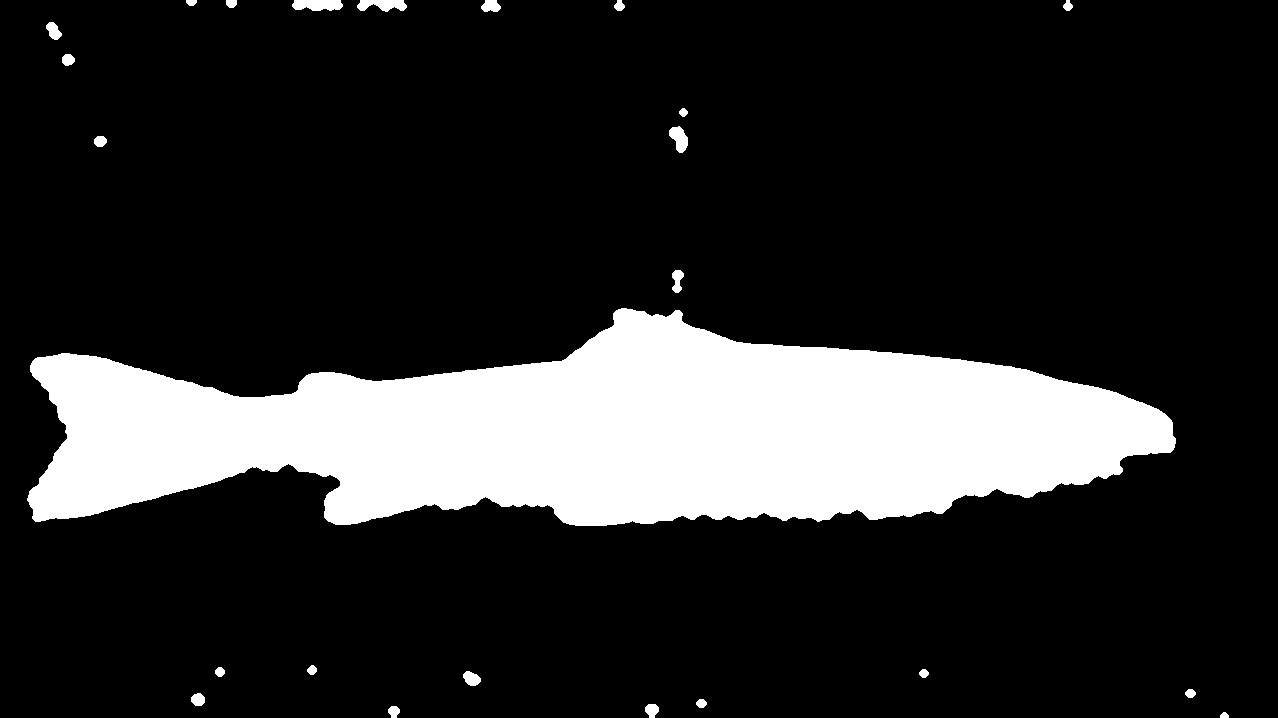
\includegraphics[width=\linewidth]{images/implementation/4_5_erode}
        \caption{Erode} 
        \label{fig:erode_contour}
    \end{subfigure}\hspace*{\fill}
    \begin{subfigure}{0.49\textwidth}
        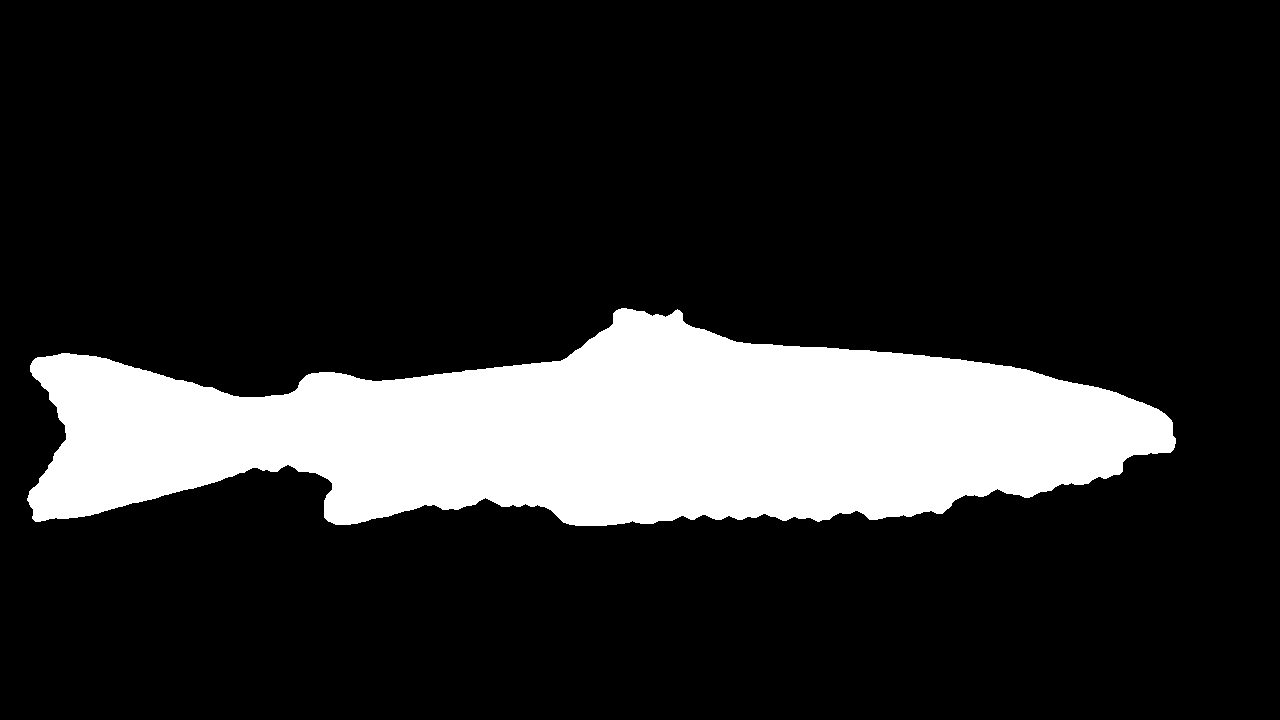
\includegraphics[width=\linewidth]{images/implementation/4_largest_contour}
        \caption{Largest Contour} 
        \label{fig:largest_contour_2}
    \end{subfigure}
    \caption{Finding the Largest Contour} 
    \label{fig:find_largest_contour}
\end{figure}


\begin{figure}[H]
    \begin{subfigure}{0.49\textwidth}
        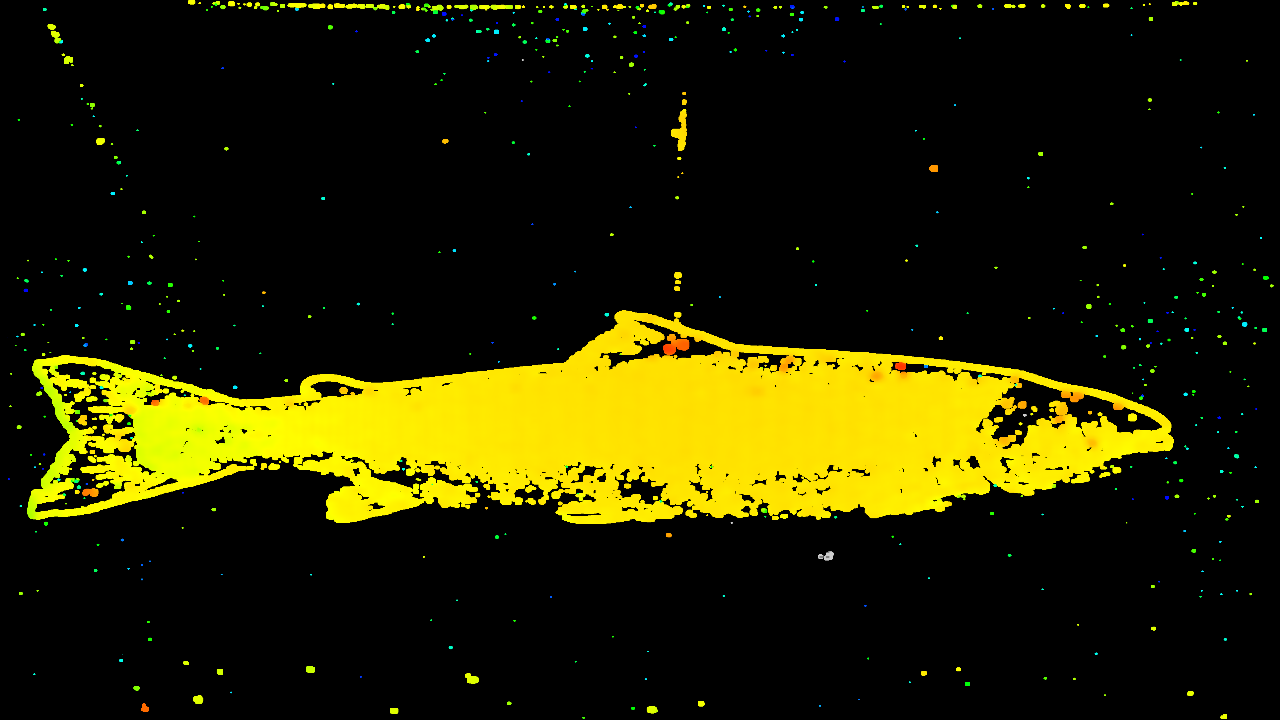
\includegraphics[width=\linewidth]{images/implementation/1_original}
        \caption{Original depthmap image} 
        \label{fig:original_depthmap}
    \end{subfigure}\hspace*{\fill}
    \begin{subfigure}{0.49\textwidth}
        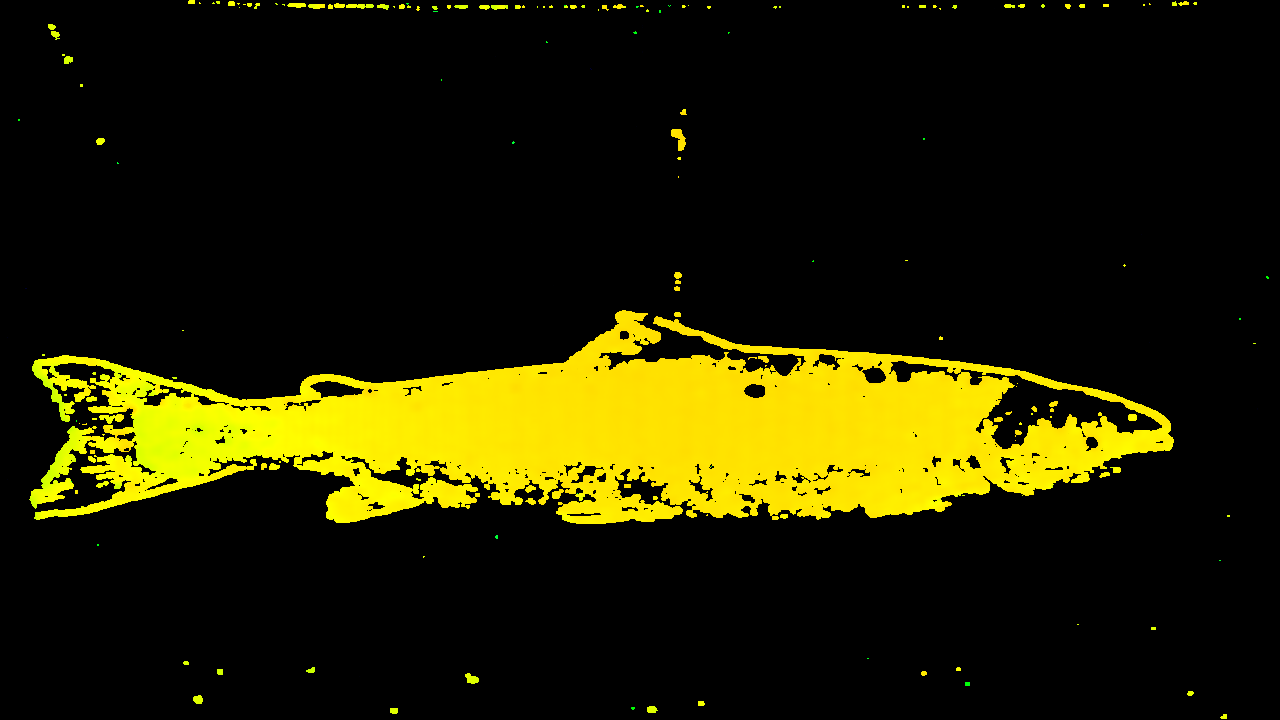
\includegraphics[width=\linewidth]{images/implementation/2_color_filtering}
        \caption{Color-Filtered Image} 
        \label{fig:color_filtering}
    \end{subfigure}
    
    \medskip
    \begin{subfigure}{0.49\textwidth}
        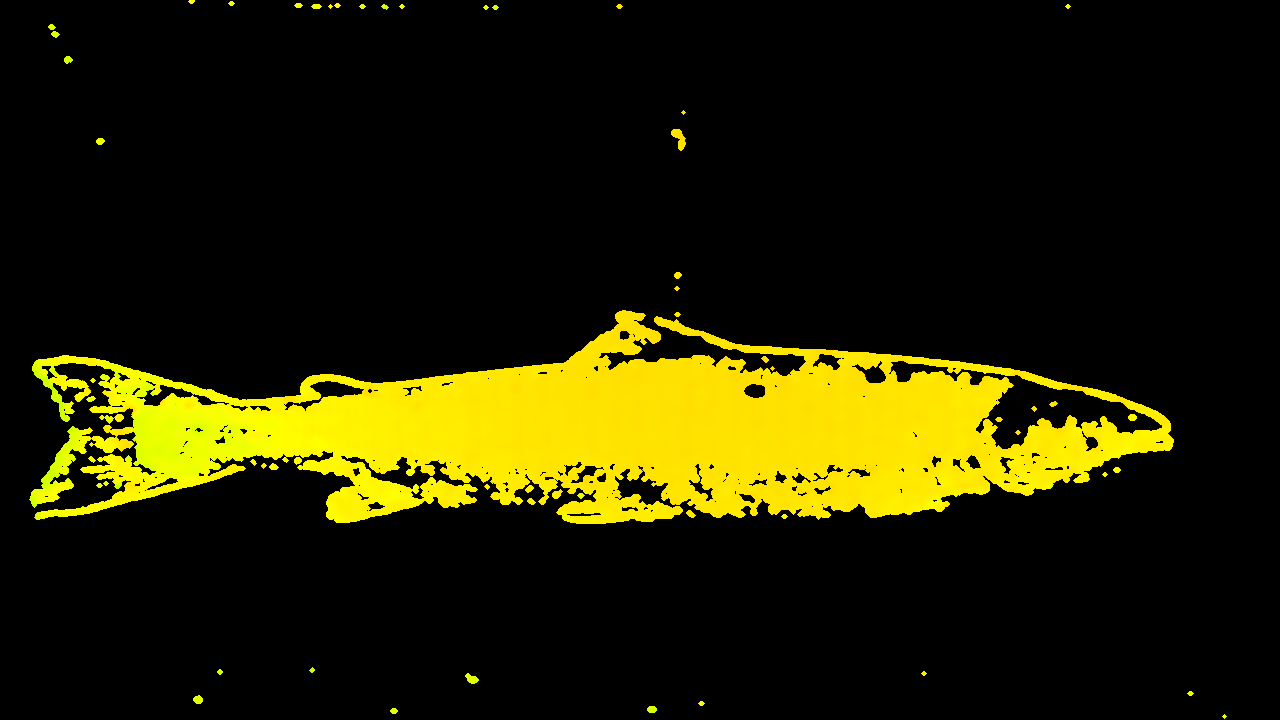
\includegraphics[width=\linewidth]{images/implementation/3_remove_particles}
        \caption{Removal of Small Particles} 
        \label{fig:remove_particles}
    \end{subfigure}\hspace*{\fill}
    \begin{subfigure}{0.49\textwidth}
        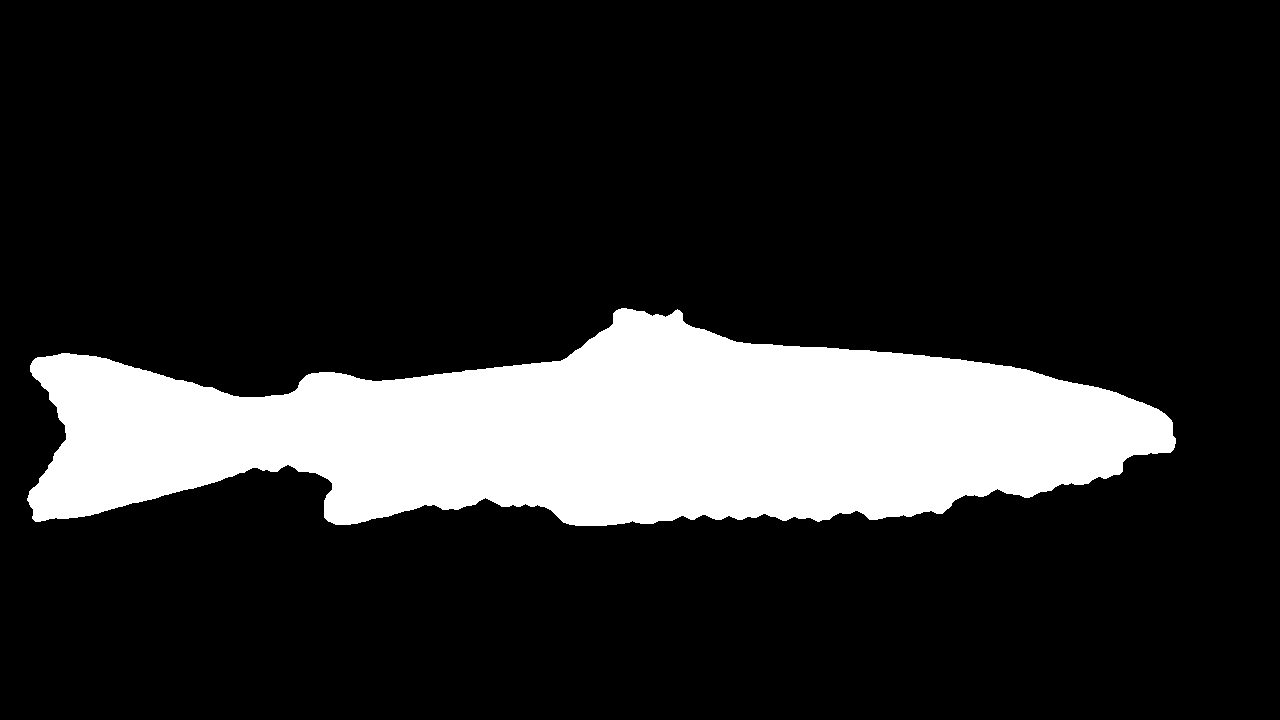
\includegraphics[width=\linewidth]{images/implementation/4_largest_contour}
        \caption{Largest Contour} 
        \label{fig:largest_contour}
    \end{subfigure}
    
    \medskip
    \begin{subfigure}{0.49\textwidth}
        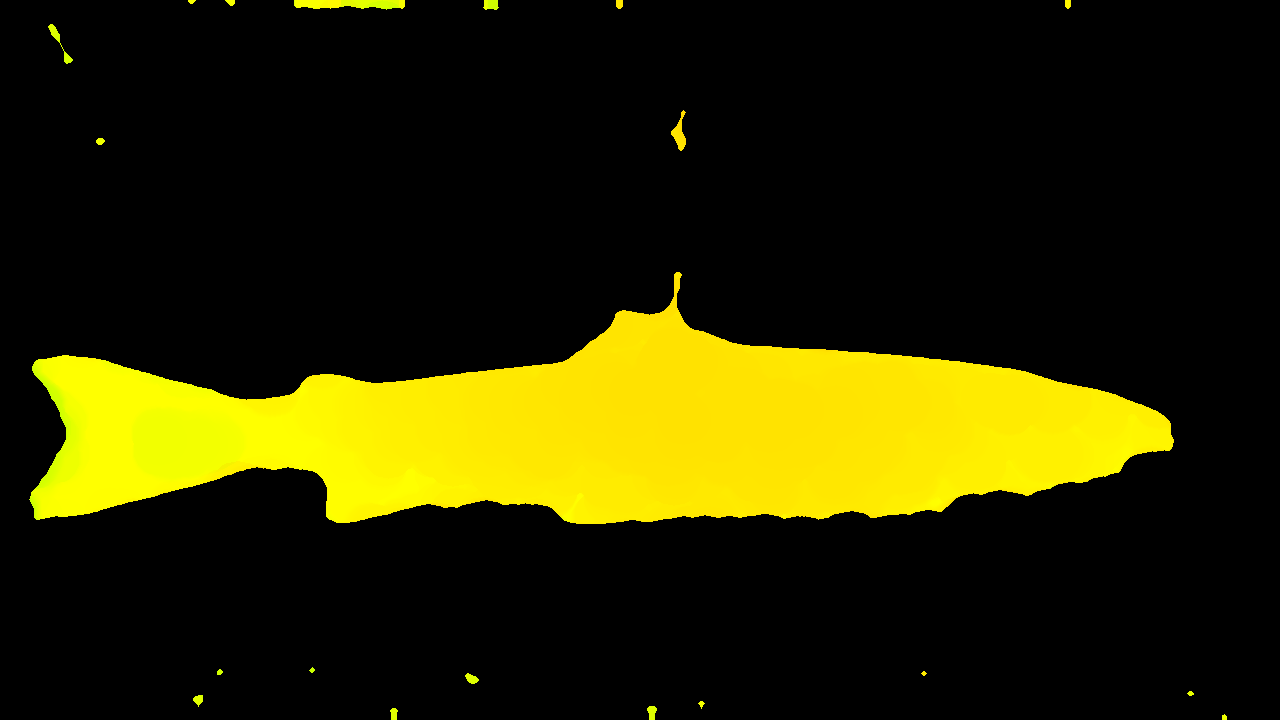
\includegraphics[width=\linewidth]{images/implementation/5_closing_on_color_filtered_image}
        \caption{Morphological Closing on (c)} 
        \label{fig:morphological_closing}
    \end{subfigure}\hspace*{\fill}
    \begin{subfigure}{0.49\textwidth}
        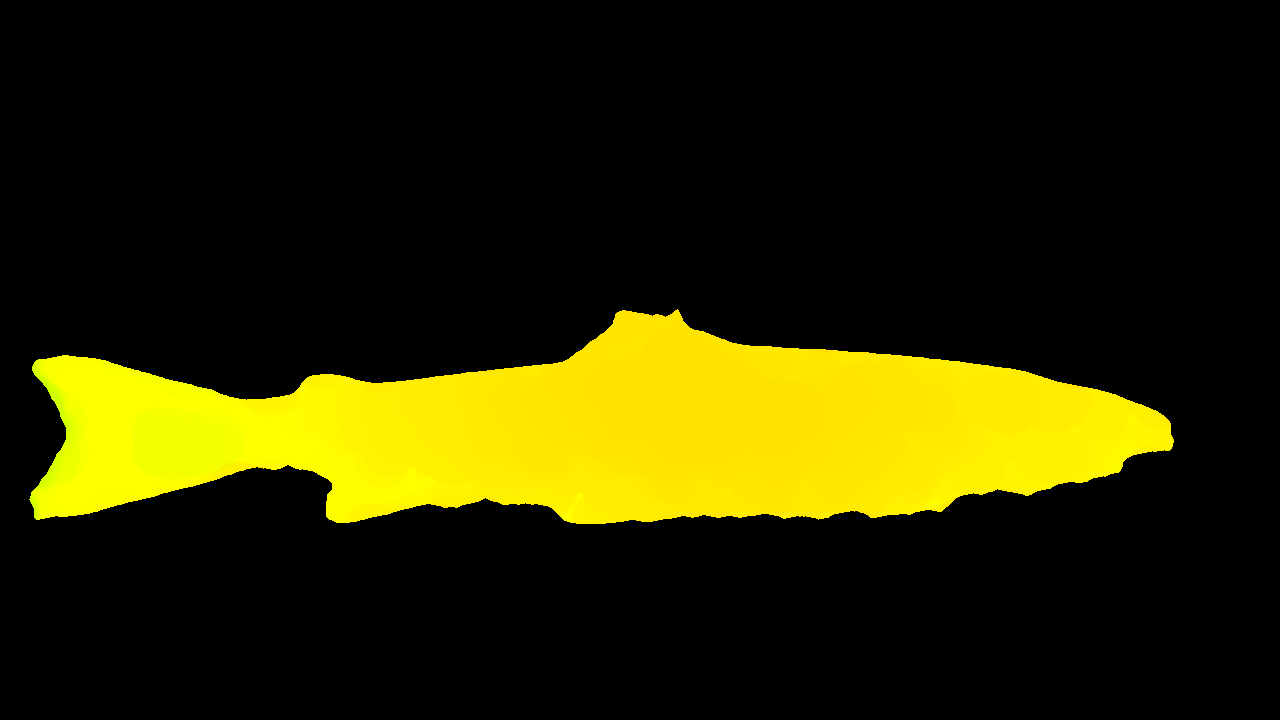
\includegraphics[width=\linewidth]{images/implementation/6_masked_source}
        \caption{Masked Image of (d) and (e)} 
        \label{fig:masked_source}
    \end{subfigure}
    \caption{Morphological Closing and Masking with Largest Contour} 
    \label{fig:algorithm}
\end{figure}



